\section{Nagios}

\subsection{Allgemein}
Nagios dient zum Überwachen von Hosts und deren Services in komplexen Infrastrukturen(Host und Services erklären?) und wurde von dem Amerikaner Ethan Galstad seit 1999\footnote{Quelle: \url{http://www.netsaint.org/changelog.php}} - damals unter der Vorgängerversion NetSaint - entwickelt und bis heute gepflegt.
Galstad gründete aufgrund der vielfältigen(ansturmmäßig) und positiven Resonanz am 9. November 2007 die "`Nagios Enterprises LLC"', welche Nagios als kommerzielle Dienstleistung anbietet.
Die Software selbst blieb weiterhin unter der freien Lizenz "`GNU General Public License version 2"'\footnote{Quelle: \url{http://www.gnu.org/licenses/old-licenses/gpl-2.0.txt}} verfügbar.
Diese erlaubt Einblick in den Programmcode und das Modifizieren der Anwendung nach eigenen Vorstellungen.

Nagios erfreut sich hoher Beliebtheit aufgrund der (bereits vorhandenen [macht kein sinn hohe beliebtheit aufgrund der großen community?]) großen Community, die Tipps, Ratschläge und auch eigene Nagios-Plugins kostenlos anbietet.
Außerdem können selbst mit geringen Programmierkenntnissen zusätzliche Skripte zur Überwachung geschrieben werden, wenn ein spezieller Anwendungsfall dies erfordert.
Warum wird Nagios engesetzt und nicht was anders -> andere kandidaten finden openview, big brother? -> das buch vom jäger verwenden!

OpenSource halt, recht einfach plugins programmierbar (auf plugin kapitel verweisen)

\newpage
\subsection{Aufbau / Architektur}


Barth schreibt über Nagios: \begin{quote}"`Die große Stärke von Nagios - auch im Vergleich zu anderen Netzwerküberwachungstools - liegt in seinem modularen Aufbau: Der Nagios-Kern enthält keinen einzigen Test, stattdessen verwendet er für Service- und Host-Checks externe Programme, die als \textit{Plugins} bezeichnet werden."'
\begin{flushright}\cite{Barth08} S. 25\end{flushright}\end{quote} 

Dieser "`Kern"' beinhaltet das komplette Benachrichtigungssystem mit Kontaktadressen und Benachrichtigungsvorgaben (Zeit, Art, zusätzliche Kriterien), die Hosts- und Servicedefinitionen inklusive deren Gruppierungen und schließlich das Webinterface.

Die eigentlichen Checks in Form der selbständigen Plugins sind abgekapselt von diesem Kern.
Siehe hierfür auch Abbildung \ref{aktivechecks}.

\begin{figure}[ht]
	\centering
	   \fbox{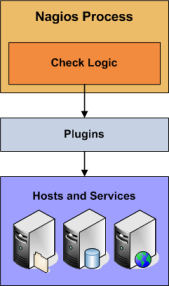
\includegraphics[scale=0.815]{bilder/activechecks.png}}
		\caption[Plugins als separate Komponente]{Plugins als separate Komponente\protect\footnote}
		\label{aktivechecks}
\end{figure} 
\footnotetext{Quelle: \url{http://nagios.sourceforge.net/docs/3_0/images/activechecks.png}}

Damit Nagios die gewünschten Server überwachen kann, müssen sie der Anwendung zuerst bekannt gemacht werden.
Dies wird über das Anlegen einer Konfigurationsdatei mit einem Host-Objekt erreicht.
Dabei richtet sich die Definition des Host-Objektes nach dem Schema, welches für alle Objektedefinitionen (Services, Kontakt, Gruppen, Kommandos etc.) gilt:

\begin{lstlisting}[captionpos=b, caption=Nagiosschema für Objektdefinitionen, label=schmeaobj, breaklines = false]
define object-type {
	parameter value
	parameter value
	...
}
\end{lstlisting}


Eine gültige Host-Definition muss mindestens folgende Elemente besitzten:

\begin{lstlisting}[captionpos=b, caption=Definition eines Hostobjektes, label=hostobj, breaklines = true, language=sh]
define host{
	host_name		example.kit.edu #Referenzname des Servers
	alias			Oracle UCM Server #Weitere Bezeichnung
	address			example.kit.edu #FQDN des Rechners
	max_check_attempts	4 #Anzahl der Checks zum Wechsel von Soft- zu Hard-State
	check_period		24x7 #Zeitraum der aktiven Checks
	contact_groups		UCM-admins #Zu alarmierende Benutzergruppe
	notification_interval	120 #Minuten bis Alarmierung wiederholt wird
	notification_period	24x7 #Zeitraum der Benachrichtigungen
}
\end{lstlisting}

In der Praxis werden öfters verwendete Attribute wie die Kontaktgruppe oder der Zeitraum für die aktiven Checks durch Verwendung eines übergeordneten Host-Objektes nach unten vererbt.
Dadurch müssen nur noch die spezifischen Informationen und der Name des übergeordneten Host-Objektes eingetragen werden.
\begin{lstlisting}[captionpos=b, caption=Verkürzte Definition eines Hostobjektes, label=vhostobj, breaklines = true, language=sh]
define host {
        use             windows-server #Oberklasse dieses Host-Objektes
        host_name       example.kit.edu
        alias           Oracle UCM Server
        address         example.kit.edu
}
\end{lstlisting}

Mit dieser Hostdefinition wird der Rechner im Webinterface von Nagios bereits angezeigt:

\begin{figure}[ht]
	\centering
	   \fbox{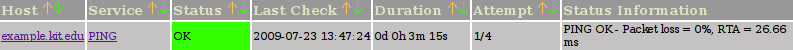
\includegraphics[width=0.9\textwidth]{bilder/example-ping.png}}
		\caption{Anzeige des Servers im Webinterface von Nagios}
		\label{check-swap}
\end{figure}

Jedoch wird nur die Erreichbarkeit über das Netzwerk mit einem Ping überwacht.
%Umfangreichere / Komplexere / Weitergehende / 
Um andere Dienste zu überwachen müssen die gewünschten Plugins explizit aus dem Nagios Repertoire dem zu überwachendem Computer mit einem ähnlichen Schema zugeteilt werden.

Eine beispielhafte Servicedefinition für die Überwachung des Webservers auf dem Host \textit{example.kit.edu} wird in Codelisting \ref{servdef} gezeigt.

\begin{lstlisting}[captionpos=b, caption=Verkürzte Definition eines Hostobjektes, label=servdef, breaklines = true, language=sh]
define service{
        use                     generic-service #Oberklasse dieses Service-Objektes
        host_name               example.kit.edu
        service_description     HTTP Server #Bezeichnung des Checks
        check_command           check_http #Angabe des Nagios-Plugins (hier ohne Parameter)
        }

\end{lstlisting}

Die Plugins werden durch die Servicedefinitionen mit den jeweiligen Hosts verbunden und durch das Attribut \textit{check\_command} mit ggf. veränderten Parametern durch Nagios aufgerufen.

Nagios wird in einem festlegbarem / veränderbarem Zeitintervall alle vom Benutzer definierten Host- und Servicechecks überprüfen und die Ergebnisse der entsprechenden Plugins verarbeiten / auswerten.

Weiterhin beschreibt Barth die Plugins folgendermaßen:
\begin{quote}"`Jedes Plugin, das bei Host- und Service-Checks zum Einsatz kommt, ist ein eigenes, selbständiges Programm, das sich auch unabhängig von Nagios benutzen lässt."' \begin{flushright}\cite{Barth08} S. 105\end{flushright}\end{quote} 

Daher lassen sich die Parameter eines Plugins folgendermaßen überprüfen:

\begin{figure}[ht]
	\centering
	   \fbox{
\includegraphics[width=0.85\textwidth]{bilder/check-swap-white.png}}
		\caption{Beispielhafte manuelle Ausführung eines Servicechecks}
		\label{check-swap}
\end{figure}

Die Ausgabe des Plugins gibt den Zustand des Services an; in diesem Fall wird kein Schwellwert überschritten, daher die Meldung \pictext{SWAP OK}.
Dieses Plugin liefert noch zusätzliche Performance-Informationen, die mit externen Programmen ausgewertet, gespeichert und visualisiert werden können.
Standardmäßig werden die Performancedaten von der normalen Ausgabe mit einem \pictext{|} getrennt.
Jedoch können auch Werte aus der normalen Textausgabe für die Visualisierung verwendet werden, so dass in diesem Beispiel keine Berechnung des Prozentsatzes notwendig wäre.

Um diesen Service mit den angegebenen Schwellwerten von Nagios überwachen zulassen, muss folgende Servicedefinition in die Konfigurationsdatei eingetragen werden:

\begin{lstlisting}[captionpos=b, caption=Beispielhafte (Definition) eines Servicechecks, label=servdef, breaklines = true, language=bash]
# Define a service to check the swap disk space
# on the local machine.  Warning if =< 20% free, 
# critical if =< 10% free space on swap partition.

define service{
 use         generic-service 
 host_name   example.kit.edu 	
 service_description  Swap Disk Space
 check_command   check_swap!-w 20% -c 10%	# Angabe des zu verwendenden Plugins mit WARNING (respektiv) CRITICAL Schwellwertparameter
}
\end{lstlisting}



Dabei wird in vier verschiedene Rückgabewerte / Antworten der Plugins unterschieden:

%\setlength{\tabcolsep}{50pt}
\begin{table}[!htbp]
\centering

\begin{tabular}{l l p{7cm}}
%\hline
\textbf{Status} \hspace{2 mm} & \textbf{Bezeichnung} \hspace{3 mm} & \textbf{Beschreibung}\\
\hline
%\textit{features} & complete\tnote{1} & complete\tnote{1} \\
%\hline
0 & OK & Alles in Ordnung \\
%\hline
1 & WARNING & Die Warnschwelle wurde überschritten, die kritische Schwelle ist aber noch nicht erreicht.\\
%\hline
2 & CRITICAL & Entweder wurde die kritische Schwelle überschritten oder das Plugin hat den Test nach einem Timeout  abgebrochen. \\
%\hline
3 & UNKNOWN &  Innerhalb des Plugins trat ein Fehler auf (zum Beispiel weil falsche Parameter verwendet wurden)\\
%\hline
\end{tabular}
\caption[Rückgabewerte für Nagios Plugins]{Rückgabewerte für Nagios Plugins\protect\footnote} %\protect\footnote
%\end{twoparttable}
\end{table}
\footnotetext{Quelle: \cite{Barth08} S. 105f}

Anhand dieser Werte wertet Nagios gezielt den Status des jeweiligen Objektes (Host oder Service) aus.
Weiterhin gibt es weiche (Soft States) und harte Zustände (Hard States):

\begin{figure}[ht]
	\centering
	   \fbox{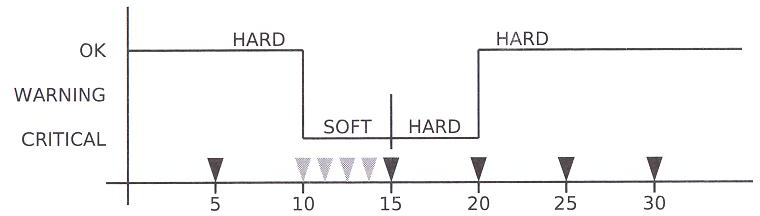
\includegraphics[width=0.85\textwidth]{bilder/hs-states.png}}
		\caption[Beispiel für den zeitlichen Verlauf durch vers. Zustände]{Beispiel für den zeitlichen Verlauf durch vers. Zustände\protect\footnote}
		\label{hs-states}
\end{figure}
\footnotetext{Quelle: \cite{Barth08} S. 95}
Ausgehend von einem OK Zustand wird in diesem Beispiel jede fünf Minuten periodisch überprüft, ob sich der Status des überwachten Objektes verändert hat.                                                                                                                                                                                         Nach zehn Minuten wird ein Umschwenken / Änderung des Zustandes durch das jeweilige Plugin gemeldet.
Hier im Beispiel wechselt der Zustand nach CRITICAL, zunächst allerdings als Soft State
Daher wird durch Nagios noch keine Benachrichtigung versendet, da es sich um eine Falschmeldung, auch False Positive genannt, handeln kann.
Aufgrund einer kurzweiligen / kurzfristigen (besseres Wort? peak mäßig) hohen Auslastung des Netzwerkes oder um ein kurzzeitiges Problem, welches sich von alleine wieder normalisiert. (Bspw. Prozessorauslastung)

Um einen False Positive auszuschließen, wird der im Soft State befindliche Service bzw. Host mit einer höheren Frequenz überprüft.
Sollten diese Überprüfungen den vorherigen Zustand bestätigen, verfestigt sich der aktuelle Zustand, man spricht nun von einem Hard State / wechselt der Zustand in den Hard State.
Erst in diesem Moment werden die entsprechenden Kontaktpersonen über den in diesem Beispiel kritischen Zustand benachrichtigt.
Sollte sich der Zustand wieder in den Normalzustand begeben und dieser Zustandsübergang wird von dem (von Nagios ausgeführten) Plugin festgestellt, wird dies an den Nagios Server gemeldet.

Ein Übergang zu dem OK Status wird sofort als Hard State festgelegt / festgehalten / festgesetzt / und führt dadurch zur sofortigen Benachrichtigung durch Nagios.

Diese Benachrichtigung

\begin{itemize}
\item Betroffene OSI Schichten auflisten und erklären
\item Wie werden die Info von Nagios gesammelt und wie gespeichert -> FlapDetection
\item FLapping \footnote{\url{http://nagios.sourceforge.net/docs/2\_0/flapping.html}}
\item Benachrichtigung durch email oder sms sogar per Telefon geht usw.
\item Hierarchie \url{http://nagios.sourceforge.net/docs/3_0/networkreachability.html}
\end{itemize}

\subsection{Service Checks und deren / ihre Realisierung / Ausführung / (Überprüfungs)Methoden}

Dienste, die im Netzwerk zur Verfügung stehen (Netzwerkdienste), wie ein Web- oder \gls{FTP}-Server , lassen sich einfach / simpel direkt über das Netz auf ihren Zustand (hin) überprüfen /  testen.
Hierfür muss dem entsprechende Plugin lediglich die Netzwerkadresse mitgeteilt werden, siehe Abbildung \ref{check-http} als beispielhafte Überprüfung eines Webservers.

\begin{figure}[ht]  
	\centering
	   \fbox{
\includegraphics[width=0.85\textwidth]{bilder/check-http.png}}
		\caption{Beispielhafte manuelle Ausführung eines netzwerkbasierenden Servicechecks / HTTP Server Check}
		\label{check-http}
\end{figure}

(Bitte beachten, dass das Plugin immernoch auf dem Nagios Server ausgeführt wird / sich immernoch auf dem Nagios Server befindet)

Dienste, die sich nicht standardmäßig / ohne weiteres / ohne weitere Anpassung(en) über das Netzwerk überprüfen lassen, wie die Kapazität einer Festplatte auf einem entfernten Server(, das (Laufen) eines Prozesses) oder die Durchsuchung einer Logdatei nach bestimmten (Stop)wörtern.

Nagios bietet verschiedene Möglichkeiten an solche Dienste /  Services zu überprüfen:

\begin{figure}[ht]
	\centering
	   \fbox{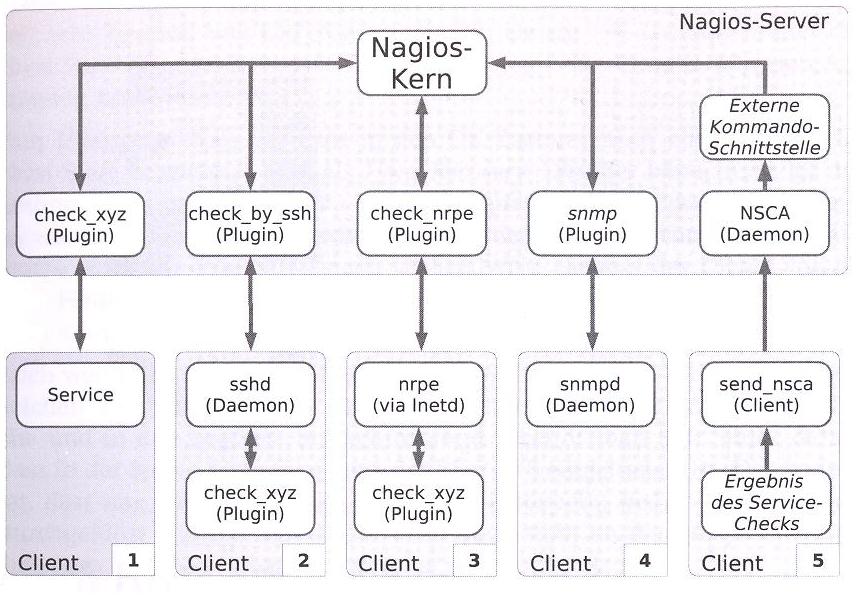
\includegraphics[width=0.85\textwidth]{bilder/nagios-kern.png}}
		\caption{Verschiedene Überwachungsmöglichkeiten von Nagios}\footnote{Quelle: \cite{Barth08} S. 98}
		\label{nagios-kern}
\end{figure} 

\textit{Hier die Zahlen als Wort oder Ziffer stehen lassen?}

\paragraph{Variante / Methode / Client 1}

Der zuvor, in Abbildung \ref{check-http}, gezeigte / abgebildete Test eines netzwerkbasierenden Dienstes wird im obigen Bild mit dem Client-Rechner (mit der Nummer) 1 realisiert.
Die Überprüfung von nicht netzwerkbasierenden Diensten soll mit den restlichen Client-Rechnern exemplarisch aufgezeigt werden.

\paragraph{Variante / Methode / Client 2}

Falls es sich beim Client um ein Unixderivat handelt, ist der entfernte Zugriff auf diesen Client per SSH\footnote{Durch eine Secure Shell (\gls{SSH}) kann man sich eine verschlüsselte Netzwerkverbindung zum entfernten Rechner aufbauen.}-Dienst möglich.
Dazu muss auf dem Client ein SSH-Benutzerkonto angelegt sein, mit dem sich Nagios anmelden kann und die öffentlichen Schlüssel (zwischen Nagios Server und Client) ausgetauscht werden, damit keine passwortabhängige Benutzerauthentifizierung (Eingabe von PW) notwendig ist.
Danach können lokale Ressourcen, wie Festplattenkapazität oder Logdateien mit dem entsprechenden Plugin direkt auf dem entfernten Rechner überwacht werden.
Damit der Client diese Plugins verwenden kann, müssen sich die gewünschten Plugins (auch) auf dem Client (lokal) befinden.
Eine beispielhafte Verwendung mit dem dafür gedachten Nagios Plugin \pictext{check\_by\_ssh} (von dieser Überwachungsmethode) wird in Abbildung \ref{check-ssh} gezeigt.

\begin{figure}[ht]
	\centering
	   \fbox{
\includegraphics[width=0.85\textwidth]{bilder/check_by_ssh.png}}
		\caption{Beispielhafte manuelle Ausführung eines Servicechecks über SSH}
		\label{check-ssh}
\end{figure}

(Hier beachten, dass kein Passwort abgefragt wird, daher zuvor Schlüsselaustauschen)

\paragraph{Variante / Methode / Client 3}

Eine alternative Möglichkeit solche Dienste auf entfernten Rechnern zu überwachen, ist durch den sogenannten Nagios Remote Plugin Executor (\gls{NRPE}).
Hier muss auf dem Client (extra) ein "`Agent"' installiert werden, welcher einen (TCP)-Port öffnet und auf diesem auf Anweisungen durch den Nagios Server horcht.

Der Nagios Server kann diese Anforderungen über das (dafür gedachte) Plugin \pictext{check\_nrpe} an den Client verschicken.
Ein Aufruf dieses Plugins ist dem des \pictext{check\_by\_ssh} Plugins, siehe dazu Abbildung \ref{check-ssh}, sehr ähnlich.

Der Nachteil dieser Variante ist ein zusätzlich geöffneter Port und der höhere / erhöhte Aufwand beim Installieren des Agenten im Gegensatz zum (vermutlich /meistens) bereits laufendem SSH-Dienst.
Zusätzlich gibt es nur die Möglichkeit die Anfragen auf diesem Port auf bestimmte IPs zu beschränken, jedoch nicht den Zugriff durch ein Passwort zu sichern.
Dafür beschränkt sich der NRPE (lediglich) auf die auf dem entfernten Client liegenden Nagios Plugins und kann nicht System- bzw. Benutzerkommandos aufrufen, wie bspw. das \pictext{rm} Kommando zum Löschen von Dateien, welches durch den Einsatz von \pictext{check\_by\_ssh} standardmäßig möglich wäre.
Daher könnte die SSH Variante (wenn unbehandelt PATH, user einschränken) fatale Folgen nach sich ziehen, wenn es ein Angreifer schafft die Kontrolle über den Nagios Server zu erlangen.
Beide Verfahren (hingegen) unterstützen die Verschlüsselung des Datenaustausches untereinander.

\paragraph{Variante / Methode / Client 4}
Diese Variante wird nur grob angerissen / kurz / verkürzt behandelt, da sich diese Arbeit hauptsächlich mit der Überwachung von Servern beschäftigt und nicht von Netzwerkkomponenten wie Switches oder Router, die nur per Simple Network Management Protocol (\gls{SNMP}) überwacht werden können, wenn mehr Informationen als eine schlichte Erreichbarkeit überprüft / gesammelt werden soll.

Barth schreibt über diese Variante / Überwachungsmethode:
\begin{quote}"`Mit dem Simple Network Management Protocol SNMP lassen sich ebenfalls lokale Ressourcen übers Netz abfragen [...]. Ist auf dem Zielhost ein SNMP-Daemon installiert [...] kann Nagios ihn nutzen, um lokale Ressourcen wie Prozesse, Festplatten oder Interface-Auslastung abzufragen."' \begin{flushright}\cite{Barth08} S. 101\end{flushright}\end{quote} 

Durch SNMP kann auf die strukturierte Datenhaltung der MIB\footnote{Die Management Information Base (\gls{MIB}) dient als SNMP-Informationstruktur und besteht aus einem hierarchischen, aus Zahlen aufgebauten Namensraum. Ähnliche Struktur wie andere hierarchische Verzeichnisdiensten wie \gls{DNS} oder \gls{LDAP}. Quelle: \cite{Barth08} S.233} in den entfernten Netzwerkknoten zugegriffen werden.

\begin{center}
TODO: SNMP MIB?
\end{center}



Man unterscheidet zwischen aktiven und passiven Checks.
\paragraph{passive}
asynchron!
Bei passiven Tests führt der zu überwachende Computer das statuserzeugende Ergebnis selbst aus und sendet es über ein Plugin zum Nagios Server.
Hierfür muss das Testprogramm bzw Script und das entsprechende Plugin \pictext{send\_ncsa}, welches zum Versenden der Informationen zuständig ist, auf dem Host vorhanden sein.
Auf der anderen Seite muss der \pictext{\gls{NSCA}} (Nagios Service Check Acceptor)  als Dämon gestartet sein, damit die übermittelten Ergebnisse entgegengenommen werden können.
\begin{figure}[ht]
	\centering
	   \fbox{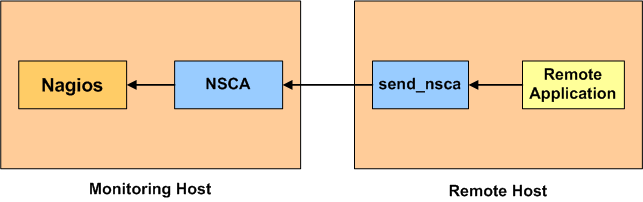
\includegraphics[width=0.85\textwidth]{bilder/nsca.png}}
		\caption{Passive Checks mit NSCA}\footnote{Quelle: http://www.nagios.org/images/addons/nsca/nsca.png}
		\label{passivchecks}
\end{figure}


\begin{figure}[ht]
	\centering
	   \fbox{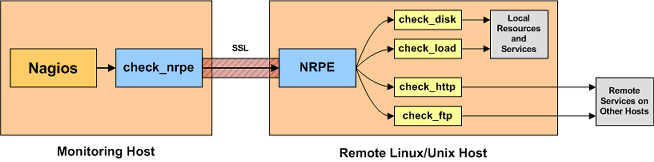
\includegraphics[width=0.9\textwidth]{bilder/nrpe.png}}
		\caption{Aktive Checks mit NRPE}\footnote{Quelle: http://www.nagios.org/images/addons/nrpe/nrpe.png}
		\label{aktivchecks}
\end{figure}
\begin{itemize}
\item Kurz agenten, zeigen auf f. Kapitel -> SNMP erklären (MIB, OID) Sicherheitsrisiko
\end{itemize}

\subsection{Überwachungslogik (mit Alarmierung/Benachrichtigung)}



\subsection{Plugins}
Gedacht für Linux umgebung

Verschiedene Möglichkeiten Checks zu realisieren unter Unix Systemen:

\begin{figure}[ht]
	\centering
	   \fbox{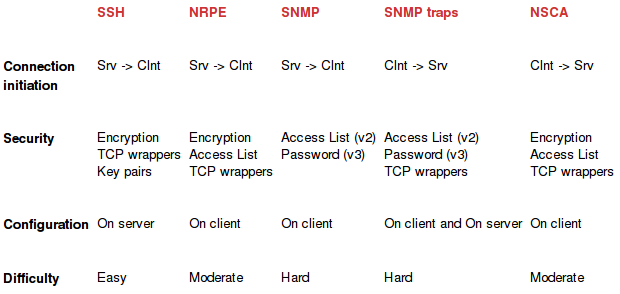
\includegraphics[width=0.9\textwidth]{bilder/unix-agents.png}}
		\caption{Übersicht der verschiedenen Unix Agenten\protect\footnotemark}
		\label{nix-agents}
\end{figure}
\footnotetext{Quelle: \url{http://www.kilala.nl/Sysadmin/index.php?id=708}}

Leicht programmierbar -> perl
Extra Plugins für Windows

\subsection{(Windows) Agenten oder allgemein Einholen von Infos}
Warum nicht einfach alles über SNMP? -> ODI muss man erst beantragen, hoher Aufwand und dann doch nicht so universell/alles abdeckend wie aktive checks, man kann keine logfiles durchuchen -> könnte es aber als standalone prog auf dem client laufen lassen und dieser sendet dann passive checks

Sagen das auf alten NSClient verzichtet wird und OpMon Agent nicht behandelt
\begin{enumerate}
\item Bilder ausm Nagios Buch Seite 472ff!
\item NSClient++
\item NC\_Net
\item NRPE\_NT
\end{enumerate}

Zusammenfassung?

\begin{figure}[ht]
	\centering
	   \fbox{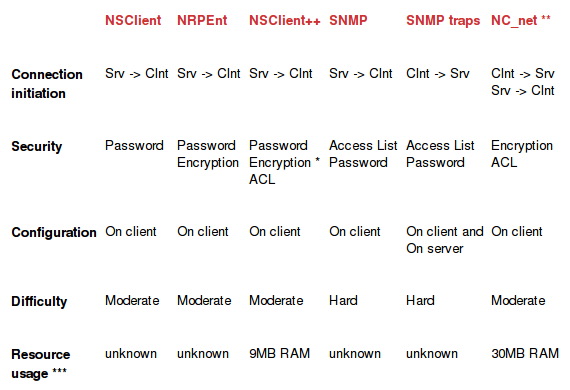
\includegraphics[width=0.9\textwidth]{bilder/win-agents.png}}
		\caption{Übersicht der verschiedenen Windows Agenten}\footnote{Quelle: \url{http://www.kilala.nl/Sysadmin/index.php?id=709}}
		\label{win-agents}
\end{figure}

Welche wird jetzt eingesetzt und warum?

Erwähne sichheitsstechnisch Parameter erlauben oder nicht erlauben

Dabei sagen, dass wenn nicht erlaubt sind keine zentrale Konfiguration der Checks auf dem Nagios server möglich ist -> abwägen

\subsection{Visualisierung der eingesammelten Daten}

